% !TEX TS-program = XeLaTeX
% use the following command:
% all document files must be coded in UTF-8
\documentclass[portuguese]{textolivre}
% build HTML with: make4ht -e build.lua -c textolivre.cfg -x -u article "fn-in,svg,pic-align"

\journalname{Texto Livre}
\thevolume{16}
%\thenumber{1} % old template
\theyear{2023}
\receiveddate{\DTMdisplaydate{2023}{5}{8}{-1}} % YYYY MM DD
\accepteddate{\DTMdisplaydate{2023}{8}{9}{-1}}
\publisheddate{\DTMdisplaydate{2023}{10}{15}{-1}}
\corrauthor{Rafael Lira Gomes Bastos}
\articledoi{10.1590/1983-3652.2023.46126}
%\articleid{NNNN} % if the article ID is not the last 5 numbers of its DOI, provide it using \articleid{} commmand 
% list of available sesscions in the journal: articles, dossier, reports, essays, reviews, interviews, editorial
\articlesessionname{articles}
\runningauthor{Bastos} 
%\editorname{Leonardo Araújo} % old template
\sectioneditorname{Daniervelin Pereira}
\layouteditorname{João Mesquita}

\title{Os memes e a polêmica velada sobre o ensino remoto emergencial}
\othertitle{The memes and the hidden polemic about emergency remote teaching}
% if there is a third language title, add here:
%\othertitle{Artikelvorlage zur Einreichung beim Texto Livre Journal}

\author[1]{Rafael Lira Gomes Bastos~\orcid{0000-0002-6828-5976}\thanks{Email: \href{mailto:lira.bastos@uece.br}{lira.bastos@uece.br}}}
\affil[1]{Universidade Estadual do Ceará, Faculdade de Educação e Ciências Integradas do Litoral Leste, Fortaleza, CE, Brasil.}

\addbibresource{article.bib}
% use biber instead of bibtex
% $ biber article

% used to create dummy text for the template file
\definecolor{dark-gray}{gray}{0.35} % color used to display dummy texts
\usepackage{lipsum}
\SetLipsumParListSurrounders{\colorlet{oldcolor}{}.\color{dark-gray}}{\color{oldcolor}}

% used here only to provide the XeLaTeX and BibTeX logos
\usepackage{hologo}

% if you use multirows in a table, include the multirow package
\usepackage{multirow}

% provides sidewaysfigure environment
\usepackage{rotating}


% CUSTOM EPIGRAPH - BEGIN 
%%% https://tex.stackexchange.com/questions/193178/specific-epigraph-style
\usepackage{epigraph}
\renewcommand\textflush{flushright}
\makeatletter
\newlength\epitextskip
\pretocmd{\@epitext}{\em}{}{}
\apptocmd{\@epitext}{\em}{}{}
\patchcmd{\epigraph}{\@epitext{#1}\\}{\@epitext{#1}\\[\epitextskip]}{}{}
\makeatother
\setlength\epigraphrule{0pt}
\setlength\epitextskip{0.5ex}
\setlength\epigraphwidth{.7\textwidth}
% CUSTOM EPIGRAPH - END

% LANGUAGE - BEGIN
% ARABIC
% for languages that use special fonts, you must provide the typeface that will be used
% \setotherlanguage{arabic}
% \newfontfamily\arabicfont[Script=Arabic]{Amiri}
% \newfontfamily\arabicfontsf[Script=Arabic]{Amiri}
% \newfontfamily\arabicfonttt[Script=Arabic]{Amiri}
%
% in the article, to add arabic text use: \textlang{arabic}{ ... }
%
% RUSSIAN
% for russian text we also need to define fonts with support for Cyrillic script
% \usepackage{fontspec}
% \setotherlanguage{russian}
% \newfontfamily\cyrillicfont{Times New Roman}
% \newfontfamily\cyrillicfontsf{Times New Roman}[Script=Cyrillic]
% \newfontfamily\cyrillicfonttt{Times New Roman}[Script=Cyrillic]
%
% in the text use \begin{russian} ... \end{russian}
% LANGUAGE - END

% EMOJIS - BEGIN
% to use emoticons in your manuscript
% https://stackoverflow.com/questions/190145/how-to-insert-emoticons-in-latex/57076064
% using font Symbola, which has full support
% the font may be downloaded at:
% https://dn-works.com/ufas/
% add to preamble:
% \newfontfamily\Symbola{Symbola}
% in the text use:
% {\Symbola }
% EMOJIS - END

% LABEL REFERENCE TO DESCRIPTIVE LIST - BEGIN
% reference itens in a descriptive list using their labels instead of numbers
% insert the code below in the preambule:
%\makeatletter
%\let\orgdescriptionlabel\descriptionlabel
%\renewcommand*{\descriptionlabel}[1]{%
	%  \let\orglabel\label
	%  \let\label\@gobble
	%  \phantomsection
	%  \edef\@currentlabel{#1\unskip}%
	%  \let\label\orglabel
	%  \orgdescriptionlabel{#1}%
	%}
%\makeatother
%
% in your document, use as illustraded here:
%\begin{description}
%  \item[first\label{itm1}] this is only an example;
%  % ...  add more items
%\end{description}
% LABEL REFERENCE TO DESCRIPTIVE LIST - END


% add line numbers for submission
%\usepackage{lineno}
%\linenumbers

\begin{document}
	
\maketitle
	
\begin{polyabstract}
\begin{abstract}
O objetivo deste artigo é analisar a polêmica velada veiculada por \textit{memes} sobre o ensino remoto emergencial, vivenciado durante a pandemia de COVID-19 no Brasil. Para tanto, por meio do aporte teórico-metodológico da Análise Dialógica do Discurso, especialmente da noção de polêmica velada, analisamos três \textit{memes} que circularam nas redes sociais durante os anos de 2020 e 2021. Os resultados apontam que os autores dos \textit{memes} utilizam a polêmica velada como uma forma de hostilizar aspectos dos denominados discursos capitalista, pedagógico tradicional e tecnológico. Dessas relações dialógicas, são produzidos sentidos, efeitos de sentidos, que vão em direção a uma crítica social mais ampla. Essa crítica revela tanto as fragilidades do ensino remoto emergencial quanto as desigualdades sociais que dificultaram a sua viabilidade.
			
\keywords{Memes \sep Polêmica velada \sep Ensino remoto emergencial}
\end{abstract}
		
\begin{english}
\begin{abstract}
The purpose of this article is to analyze the hidden polemic conveyed by memes about the emergency remote teaching, experienced during the COVID-19 pandemic in Brazil. To this end, we analyzed three memes that circulated on social networks during the years 2020 and 2021, through the theoretical-methodological contribution of Dialogical Discourse Analysis, especially the notion of hidden polemic. The results indicate that the authors of the memes use the hidden polemic as a way of confronting aspects of the so-called capitalist, traditional pedagogical and technological discourses. Meanings and effects of meanings are produced by these dialogical relationships, which go towards a broader social critique. This criticism reveals both the weaknesses of emergency remote teaching and the social inequalities that hindered its viability.
				
\keywords {Memes \sep Hidden polemic \sep Emergency remote teaching}
\end{abstract}
\end{english}
% if there is another abstract, insert it here using the same scheme
\end{polyabstract}
	
\section{Introdução}\label{sec-intro}
A pandemia de covid-19 surgiu no ano de 2020, acarretando, além da necessidade de isolamento social para a preservação da vida, sofrimento e morte. O Brasil, por exemplo, aparece como o segundo país no mundo com o maior número de mortes devido à infecção causada pelo vírus \cite{souzajunior2021transmediatisation}. Não bastasse o problema sanitário, instalou-se no país uma crise política sem precedentes, na qual o próprio presidente da república colocava em dúvida a gravidade da doença, a necessidade de isolamento social e, futuramente, a eficácia das vacinas, provocando um verdadeiro caos na saúde pública \cite{dias2021maismedicos}. Diante dessa situação, os estudiosos da linguagem começaram a refletir sobre o tema, notadamente sobre o impacto das \textit{fake news} na vida das pessoas como uma forma de registrar e, ao mesmo tempo, denunciar o complicado momento histórico que vivenciávamos \cite{lima2021producao,recuero2021discurso}.

Concomitante a esse cenário desolador provocado pela doença, as escolas de educação básica e as universidades brasileiras, na sua maioria, decidiram pela continuidade das aulas de forma remota. Quase que no improviso e sem a formação necessária, os professores viram-se obrigados a mudar completamente o formato de realização de sua atividade de ensino. O ensino remoto emergencial (doravante, ERE), assim, passou a ser uma realidade em meio às incertezas provocadas pela situação sanitária. Apesar disso, os professores foram acusados, pelo mesmo Governo Federal, de não trabalharem durante a pandemia. Como consequência, instaurou-se um discurso de ódio sem precedentes contra a categoria nas redes sociais \cite{araujo2022projeto}.
	
Mesmo assim, os professores continuaram seu trabalho que, diga-se de passagem, nunca parou, nem na sala de aula e nem na pesquisa acadêmica. Alguns esforços, inclusive de nossa parte, foram feitos na tentativa de compreender melhor o ERE \cite{bastos2020narrativas,bastos2021interacoes,paes2020trabalho,costa2022estudo}. Por meio desses estudos, o ERE foi caracterizado, do ponto de vista dos alunos, como controverso; se, por um lado, os alunos sofreram pela falta de conectividade, por outro lado, houve certo ganho na busca pela autonomia da aprendizagem \cite{bastos2020narrativas}. Do ponto de vista do professor, o ERE se destacou como desafiador, uma vez que faltou formação adequada e acesso à internet que pudesse garantir a participação de todos os alunos nas aulas \textit{on-line} \cite{paes2020trabalho}. 

 
Durante a situação emergencial, o campo da atividade educacional produziu inúmeras formas de tematizar o ERE. Algumas delas foram feitas com bastante humor e/ou ironia, como é o caso dos \textit{memes} que circularam nas redes sociais e que rapidamente se tornaram objeto de estudo. \textcite{maddalena2020meme}, por exemplo, concluíram que os \textit{memes} criticavam a leitura do livro didático pelo professor e a falta de interesse dos alunos em participar das aulas. Já na Linguística Aplicada (LA), \textcite{lima2022reflexao} apresentou uma (auto) reflexão sobre uma aula remota de língua inglesa por meio da análise de \textit{memes}, demonstrando as relações dialógicas entre o texto e a imagem na composição do enunciado verbo-visual. Além disso, ainda que de forma preliminar, o autor também destacou algumas relações dialógicas polêmicas entre o \textit{meme}, o ensino remoto emergencial e as condições de acesso às tecnologias no contexto da escola pública.
	
Inserido nesse diálogo, portanto, tenho como objetivo analisar a polêmica velada veiculada por \textit{memes} sobre o ensino remoto emergencial, vivenciado durante a pandemia de COVID-19 no Brasil. Ampliando o estudo de \textcite{lima2022reflexao}, considero, para isso, o aporte teórico-metodológico da Análise Dialógica do Discurso (ADD), recorrendo, especialmente, à noção de polêmica velada, como discutida em \textcite{bakhtin2018problemas}. Para dar conta do objetivo, selecionei para a análise três exemplares de \textit{memes} que circularam nas redes sociais nos anos de 2020 e 2021. Assim, amparado na ideia de \textcite{bakhtin2018problemas} de que os sentidos se distribuem em torno de diferentes vozes sociais, este estudo pode contribuir para ampliar a discussão sobre a análise da polêmica velada nos discursos de diferentes campos da atividade humana, como sugerido por \textcite{silva2019analise} e \textcite{campos2021concepcao}. Da mesma forma, pode contribuir para registrar historicamente o ERE por meio das produções de sentido veiculadas pelos \textit{memes}, já que, ao recuperarmos as (des)aprendizagens vivenciadas naquele momento, podemos projetar futuros possíveis, a partir do que pode ser (des)favorável para as práticas educativas atuais.
	
O artigo está organizado da seguinte forma: além desta introdução, na próxima seção, são discutidas a metalinguística de Bakhtin e a noção da polêmica velada; em seguida, o \textit{meme} é caracterizado como um enunciado verbo-visual do ponto de vista dialógico; a metodologia da pesquisa é detalhada; é realizada a análise dialógica da polêmica velada nos \textit{memes} e, por fim, são apresentadas as considerações finais.
	
\section{A metalinguística de Bakhtin e a noção da polêmica velada}\label{sec-metalingBaktin}
Ao realizar uma importante e criteriosa historicização sobre a publicação e a recepção dos textos de Bakhtin e o Círculo no Brasil, demonstrando como consolidou-se a Análise Dialógica do Discurso, \textcite{portoboenavides2022publicacao} defende a ideia de que é necessário considerar-se, nas análises desenvolvidas, tanto o projeto de Bakhtin para a criação da metalinguística, como uma nova disciplina para o campo do discurso, como a produção intelectual dos pesquisadores brasileiros sobre as ideias dos autores russos. Seguindo o entendimento da autora, pretendo, nesta seção, desenvolver um caminho teórico a partir da metalinguística em diálogo com os pesquisadores brasileiros, especialmente com aqueles que se dedicam ao estudo, ainda preliminar, da polêmica velada nos discursos cotidianos \cite{silva2019analise,campos2021concepcao}.
	
O projeto da criação da metalinguística, ao que deixa implícito a leitura das obras de Bakhtin e o Círculo, de acordo com \textcite{silva2019analise}, foi iniciado desde uma das primeiras produções de \textcite{bakhtin2017filosofia}, \textit{Por uma filosofia do ato responsável}, ainda na década de 1920. O projeto ganhará consolidação, contudo, durante a década de 1960 e é melhor sistematizado na segunda edição do livro \textit{Problemas da poética de Dostoiévski} \cite{bakhtin2018problemas}, publicado, na Rússia, em 1963. Especialmente no capítulo intitulado \textit{O discurso em Dostoiévski}, Bakhtin explica pormenorizadamente o motivo pelo qual defende a necessidade dessa nova disciplina para o estudo do discurso em geral e do discurso literário em específico.
	
A metalinguística pode ser compreendida como uma disciplina com um objeto próprio, que investiga o campo da vida do discurso. No contexto brasileiro, em minha interpretação, o conhecimento produzido pela ADD engloba a metalinguística pensada por Bakhtin, mas vai além, pois considera em seu arcabouço teórico-metodológico também as provocações do método sociológico de análise linguística desenvolvido por \textcite{volochinov2018marxismo}, bem como a poética sociológica pensada por \textcite{medvedev2012metodo}. Sem desconsiderar as contribuições dos demais autores do Círculo para a consolidação da ADD no Brasil, e tendo em vista o objetivo do artigo, gostaria de focar precisamente nas ideias de Bakhtin.
	
Quero chamar a atenção para o fato de que, na ideia do autor russo, a metalinguística diferencia-se da linguística, no sentido rigoroso do termo, justamente porque possui outro objeto (ou um objeto próprio) de investigação, qual seja, as relações dialógicas. Sobre as relações dialógicas, Bakhtin explica que

\begin{quote}    
 [...] as relações dialógicas são extralinguísticas. Ao mesmo tempo, porém, não podem ser separadas do campo do \textit{discurso}, ou seja, da língua como fenômeno integral concreto. A linguagem só vive na comunicação dialógica daqueles que a usam. É precisamente essa comunicação dialógica que constitui o verdadeiro campo da \textit{vida} da linguagem. \cite[p.~209, grifos no original]{bakhtin2018problemas}.	
\end{quote}

	
	
É preciso reafirmar que as relações dialógicas, apesar de serem impossíveis sem o material linguístico e seus elementos léxico-semânticos, só podem acontecer quando a língua se materializa em um enunciado concreto. O enunciado, para \textcite{bakhtin2016generos}, é um elo na cadeia da comunicação discursiva e se relaciona retrospectivamente e prospectivamente com outros enunciados. Além disso, Bakhtin, em diferentes textos \cite{bakhtin2016generos, bakhtin2018problemas}, insiste no fato de que todo enunciado tem um autor. Por mais que não saibamos nada sobre o autor real do enunciado, sentimos (eu diria, interpretamos, no caso da análise que desenvolvo) sua presença a partir de seu juízo de valor a respeito de um determinado objeto de discurso.
	
Isso implica que defendo, desde já, a ideia de que o \textit{meme}, como um enunciado concreto, não pode ser interpretado como um texto sem autor, por mais que não saibamos quem, de fato, assina sua produção. Isso seria um \textit{contradictio in adjecto}, pois, de acordo com \textcite[p.~72]{bakhtin2016generos}, todo enunciado “tem um sujeito, um autor (o falante ou quem escreve)”. Segundo ainda o autor russo, a linguística pode até abstrair inteiramente a autoria em suas análises, mas isso não é o caso da metalinguística, que, ao contrário, nunca desconsidera esse elemento, pois ele está ligado ao projeto de discurso de quem enuncia que, repito, pode não ser conhecido como sujeito real no mundo da vida, mas sempre é percebido, em alguma dimensão, por meio das relações dialógicas entre os enunciados.
	
Além disso, todo enunciado se realiza em torno de um projeto de discurso que, por sua vez, está relacionado a uma determinada intenção do autor, isto é, uma “relação subjetiva emocionalmente valorativa do falante com o conteúdo do objeto e do sentido do seu enunciado” \cite[p.~47]{bakhtin2016generos}. Por isso, não podemos perder de vista que o aspecto axiológico da linguagem é presença marcante nas obras do Círculo, já que não existe, segundo \textcite{bakhtin2016generos}, palavra que seja neutra, que seja dita sem um posicionamento valorativo de quem a enuncia. Diante do posicionamento axiológico\footnote{Posicionamento axiológico, expressividade, ponto de vista, tom emotivo-volitivo são termos sinônimos no conjunto da obra de Bakhtin e o Círculo.} assumido pelo locutor em um enunciado, podemos reagir dialogicamente a ele de diferentes formas, concordando, discordando, complementando-o etc. \textcite{bakhtin2018problemas}. Essa dinâmica, portanto, não pode ser diferente no caso do \textit{meme}, um enunciado que é produzido por um autor em determinadas condições e que, por consequência, tem um posicionamento valorativo a respeito do objeto de discurso que é tematizado. Voltarei a essa discussão mais tarde.
	
Dessa forma, só podem existir relações dialógicas entre enunciados ou entre elementos composicionais do mesmo enunciado, isto é, no campo da vida do discurso. Elas são possíveis, esclarece \textcite{bakhtin2018problemas}, entre dois enunciados diferentes, entre estilos, ou, até mesmo, entre palavras de um mesmo enunciado, desde que nela ouçamos a voz do outro, o ponto de vista do outro. Isso quer dizer que as relações dialógicas pressupõem sujeitos que, ao enunciar, põem em relação (de concordância ou discordância) pelo menos dois pontos de vista, duas vozes, sobre um determinado objeto de discurso. Em suma, a definição que temos defendido em trabalhos anteriores é que as relações dialógicas são relações entre sujeitos via discurso \cite{maciel2017indistincao, bastos2022disputas}.
	
Como sabemos, toda a análise realizada por Bakhtin sobre o livro anteriormente mencionado é feita com o fito de estudar as manifestações linguístico-discursivas próprias da prosa de Dostoiévski, em especial do romance polifônico. Todavia, Bakhtin, em nenhum momento, exclui a possibilidade da utilização de suas ideias na análise dos discursos da vida prática. Por isso mesmo, ele afirma que “toda a vida da linguagem, seja qual for seu campo de emprego (a linguagem cotidiana, a prática, a científica, a artística, etc.), está impregnada de relações dialógicas” \cite[p.~209]{bakhtin2018problemas}. Assim, a ADD que pratico continua o projeto de Bakhtin por meio de outras ressonâncias, ampliando sua discussão para a interpretação dos discursos que são produzidos, por exemplo, no campo educacional.
	
Mesmo ao analisar especificamente o discurso \textit{bivocal} como manifestação das relações dialógicas no contexto da relação entre o discurso do autor, do narrador e das personagens em Dostoiévski, \textcite[p. 223, grifos meus]{bakhtin2018problemas} não esquece de ponderar que “as palavras do outro, introduzidas na nossa fala, são revestidas inevitavelmente de algo novo, da nossa compreensão e da nossa avaliação, isto é, tornam-se \textit{bivocais}. [...] O nosso discurso da vida prática está cheio de palavras de outros”. Dessa forma, não preciso ir além para demonstrar, até mesmo para os bakhtinianos mais ortodoxos, que o discurso da vida prática, isto é, o discurso não literário, também pode ser submetido a uma análise \textit{bivocal} em sentido amplo, ou seja, examinando as relações dialógicas de forma geral, bem como em sentido restrito, o que permite afirmar que podemos, ao mesmo tempo, analisar a manifestação da polêmica velada em discurso de diferentes campos da atividade humana, assim como têm defendido \textcite{silva2019analise} e \textcite{campos2021concepcao}, por exemplo.
	
A polêmica velada, por seu turno, como uma manifestação tipológica do discurso \textit{bivocal} – aquele em que ouvimos duas vozes, a do autor e a da personagem, no contexto literário, ou a de dois sujeitos, no discurso cotidiano – é definida por \textcite{bakhtin2018problemas} como uma relação entre duas vozes, dois discursos, que acontece de forma subentendida.

\begin{quote}
Na polêmica velada o discurso do autor está orientado para o seu objeto, como qualquer outro discurso; neste caso, porém, qualquer afirmação sobre o objeto é construída de maneira que, além de resguardar seu próprio sentido objetivo, ela possa atacar polemicamente o discurso do outro sobre o mesmo assunto e a afirmação do outro sobre o mesmo objeto. Orientado para o seu objeto, o discurso se choca no próprio objeto com o discurso do outro. Este último não se reproduz, é apenas subentendido \cite[p.~224]{bakhtin2018problemas}.
\end{quote}
 
Prosseguindo, podemos reafirmar que, na polêmica velada, o discurso alheio não penetra de forma direta no discurso do autor do enunciado. Cabe ao analista, assim, \textit{ouvir} e interpretar a sensação da presença do discurso do outro na polêmica velada. Dessa forma, o discurso polêmico, mesmo sendo um discurso \textit{bivocal}, tem uma materialidade especial, e requer de quem analisa uma sensibilidade em ouvir as vozes que, mesmo distantes, tocam-se dialogicamente. Nessa dinâmica, a voz do autor do enunciado avalia de forma indireta e hostil o mesmo objeto de discurso como uma reação-resposta ao discurso do outro. Portanto, “em um enunciado polêmico, pode-se observar como a palavra do outro é inferida e traduzida pelo eu, bem como seus efeitos de sentido” \cite[p.~161]{silva2019analise}.

No caso da pesquisa em tela, pretendo discutir, na análise, como os \textit{memes}, considerados enunciados verbo-visuais, reagem polemicamente, mesmo que de forma velada, aos discursos que atravessam o ERE. Fazer isso pode contribuir para continuar o projeto de desenvolvimento da metalinguística de Bakhtin, e, por isso, pôr em evidência os aspectos sócio-históricos que penetram a constituição discursiva da realidade social sobre o ERE no contexto brasileiro. Para tanto, na próxima seção, apresento com mais detalhes a compreensão dos \textit{memes} como enunciados verbo-visuais.
	
\section{O \textit{meme} como um enunciado verbo-visual}\label{sec-verbo-visual}
Com a popularização das redes sociais, alguns enunciados próprios do ambiente digital começaram a circular de forma bastante viral. Dentre eles, podemos destacar o \textit{meme} que, segundo \textcite{silva2016memes}, tem se manifestado de forma avassaladora por ser uma maneira de expressão humorística dos sujeitos em relação aos diversos campos da atividade humana em que estão inseridos. Nessa perspectiva, \textcite{Bessa2023} afirmam que o \textit{meme} cumpre diversas funções no ambiente da cultura digital. Além de produzirem humor e/ou ironia, os \textit{memes},segundo os autores, funcionam como formadores de opinião, tematizando aspectos da vida política, religiosa, educacional, entre outros.
	
Como um enunciado que emerge do contexto digital, o \textit{meme} passou a ser objeto de análise de várias áreas do conhecimento, como, por exemplo, a da comunicação social \cite{recuero2008memes} e a da educação \cite{maddalena2020meme}. No caso específico dos estudos da linguagem, os \textit{memes} também são objetos de estudo e podem ser analisados em diferentes perspectivas teóricas. Nesse contexto, podemos destacar, aqui, os estudos de \textcite{souzajunior2015selfienaurna,souzajunior2016lado} que, a partir da semiótica social e da análise crítica do discurso, analisam como os \textit{memes} funcionam linguisticamente e como propagam temas políticos e/ou sociais nas interações em ambiente digital.
Não obstante a isso, a análise dos \textit{memes} não tem passado despercebida aos olhos da Análise Dialógica do Discurso em contexto brasileiro. Recentemente, \textcite{lara2020meme,lima2022reflexao,Bessa2023}, apenas para citar um recorte, utilizam as ideias de Bakhtin e o Círculo para interpretar linguístico-discursivamente o funcionamento dos \textit{memes}. No primeiro estudo, os autores investigaram a presença dos \textit{memes} em livros didáticos de português; no segundo, como os \textit{memes} podem ser usados em uma aula de língua inglesa durante o ensino remoto emergencial; e, no terceiro, as formas como os \textit{memes} expressam as representações sobre a escrita de trabalhos de conclusão de curso de alunos de graduação.
	
Amparado, portanto, nesses estudos, discuto com mais detalhes, de agora em diante, as características do \textit{meme},compreendido, aqui, como um enunciado verbo-visual, do ponto de vista dialógico. Destaco, contudo, que \textcite{souzajunior2016lado} também caracteriza o \textit{meme} como um enunciado verbo-visual, mas o autor o faz por meio de outra perspectiva teórica, o que implica uma forma de análise diferente da nossa. Na tradição dos estudos dialógicos no Brasil, é importante esclarecer que existe, há mais de quinze anos, um campo de estudo que foca precisamente na análise da verbo-visualidade (sobre isso, ver \textcite{brait2013olhar}). Os estudos da verbo-visualidade defendem a ideia de que a partir da leitura de Bakhtin e o Círculo podemos interpretar textos que sejam verbais, visuais ou verbo-visuais. Esses estudos não buscam, como podemos perceber por meio da leitura de \textcite{brait2013olhar}, substituir, complementar e/ou contrapor os estudos realizados por meio da semiótica social ou da multimodalidade. São maneiras diferentes de interpretar a relação entre a linguagem verbal e a visual, e cada uma delas ocupa um lugar diferente na área mais amplas dos estudos da linguagem. Portanto, a interpretação dos \textit{memes} que realizamos neste artigo acontece a partir dos limites dessa concepção teórica.
	
Para tanto, é importante explicitar os princípios fundantes da análise de um enunciado verbo-visual em perspectiva dialógica, já que serão a lupa de análise dos \textit{memes} apresentados adiante. Em um enunciado verbo-visual,

\begin{quote}
[...] tanto a linguagem verbal como a visual desempenham papel constitutivo na produção de sentidos, de efeitos de sentido, não podendo ser separados sob pena de amputarmos uma parte do plano de expressão e, consequentemente, a compreensão das formas de produção de sentido desse enunciado, uma vez que ele se dá a ver/ler simultaneamente \cite[p.~44]{brait2013olhar}.
\end{quote}	
	
	
A autora, no mesmo texto, ainda estabelece a diferença entre dois tipos de enunciados verbo-visuais. No primeiro tipo, estão aqueles enunciados nos quais a imagem e o texto nascem juntos, ou seja, são produzidos pelo mesmo autor com uma determinada intenção. Esse é o caso, exemplifica \textcite{brait2013olhar}, do quadro do artista René Magritte. O artista apresenta a imagem de um cachimbo e uma frase-legenda logo abaixo, dizendo “isso não é um cachimbo”. Dessa forma, as duas materialidades semióticas partem de um mesmo contexto de produção, é um enunciado verbo-visual desde sua gênese. No segundo tipo, a imagem e o texto nascem separadamente, isto é, os dois elementos possuem diferentes autorias. Esse é o caso, por exemplo, de uma edição do livro \textit{O duplo}, de Dostoiévski, analisada por \textcite{brait2013olhar}, na qual imagens foram acrescidas ao texto original. Aqui, as relações dialógicas se complexificam, uma vez que precisamos considerar, além da relação entre texto e imagem, o contexto primeiro de produção das duas materialidades – a verbal e a visual – que, ao se unirem em um enunciado verbo-visual, provocam novos efeitos de sentido. 
	
No caso dos \textit{memes} que trago para a análise algo semelhante acontece. A imagem e o texto também são de autores diferentes, mas que se integram em um novo enunciado – o \textit{meme}. No caso do \textit{meme}, o texto é produzido em função da imagem e com ela se integra, como demonstrado no estudo de \textcite{lima2022reflexao}, o que é diferente do livro de Dostoiévski, no qual a imagem fora produzida após o texto e a ele integrada. Não descarto, contudo, a possibilidade de alguns \textit{memes} serem produzidos totalmente por um mesmo autor, isto é, imagem e texto criados pela mesma pessoa. Em nosso caso, isso não acontece. A imagem (de um filme, de um cachorro e de um desenho animado) que compõe os \textit{memes} em nosso \textit{corpus} circularam amplamente na sociedade, mesmo antes do ensino remoto emergencial. Dessa forma, como orienta \textcite{lima2022reflexao}, a análise das relações dialógicas nos \textit{memes} como um enunciado verbo-visual necessita considerar a resposta criativa do autor ao integrar o seu texto a uma imagem que nasceu em outro contexto de produção e com outras intenções comunicativas.  
	
O \textit{meme} é, assim, caracterizado por \textcite[p. 189]{lara2020meme} como “[...] um gênero do discurso que produz humor ligado à sua eventicidade: sua arquitetônica está sempre relacionada a um acontecimento da vida, majoritariamente atual, para a produção de sentido”. Da mesma forma, \textcite[p.~348]{silva2016memes} sustenta que o \textit{meme} “é, pois, um gênero do discurso justamente porque, assim como os demais gêneros, nasce no interior de práticas discursivas de interação humana e apresenta conteúdo temático, estilo e estrutura composicional”. Contudo, essa posição sobre o \textit{meme} ser um gênero do discurso não é unânime e tem sido questionada por algumas pesquisas. \textcite{souzajunior2015selfienaurna, limaneto2021representacoes}, por exemplo, assumem que o \textit{meme} está mais ligado a uma forma de texto e que a função comunicativa pode se realizar em diferentes gêneros, como o anúncio publicitário, a mensagem motivacional e as tiras cômicas.

Seja como for, a discussão sobre o estatuto genérico do \textit{meme}, apesar de produtiva, escapa do objetivo deste estudo, que busca analisar, precisamente, a polêmica velada veiculada por \textit{memes} sobre o ensino remoto emergencial, vivenciado durante a pandemia de COVID-19 no Brasil. Assumo, para isso, que o \textit{meme} é um enunciado verbo-visual concreto, exemplar de um gênero do discurso, assim como todo enunciado \cite{bakhtin2016generos}. Dessa forma, explorando as características da análise de um enunciado ensinadas por \textcite{bakhtin2016generos}, considero, na análise aqui empreendida, além do tema, da composição e do estilo, a situação de produção, de circulação e de recepção para compreendermos bem os elementos extralinguísticos da arquitetônica do enunciado em questão, lembrando que a metalinguística se ocupa exatamente desses elementos, isto é, das relações dialógicas.
	
Nessa perspectiva, os \textit{memes} podem veicular diferentes conteúdos temáticos, quer dizer, diferentes objetos de discurso. Os \textit{memes} “muitas vezes parodiam, satirizam ou criticam sujeitos sociais, acontecimentos históricos, políticos etc, colocando novas vozes em cena e reacentuando outras” \cite[p. 191]{lara2020meme}. Composicionalmente, frequentemente o \textit{meme} apresenta uma imagem retangular ou quadrada, com um texto sobreposto, organizado na parte superior ou inferior da imagem \cite{lara2020meme}. Como também demonstrou \textcite{lima2022reflexao}, no caso dos \textit{memes}, o texto e a imagem não nascem juntos, mas são articulados pelo autor na busca pela produção de sentidos. As imagens podem ser retiradas de outros locais de circulação, geralmente de vídeos, de fotos ou de imagens virais; podem ser também personagens famosos de filmes e novelas ou personalidades das redes sociais.
	
A imagem é, por assim dizer, ressignificada de seu contexto original para o contexto do \textit{meme} pela vontade criativa do autor do enunciado que, a partir da articulação com os elementos verbais, pode produzir efeitos de humor e ironia \cite{silva2016memes}, concordando ou discordando de enunciados anteriores e futuros, no fluxo da interação discursiva. O estilo do \textit{meme}, por fim, tende a ser mais informal, pois está ligado majoritariamente a situações cotidianas. O plano de expressão verbal é usado, muitas vezes, de forma objetiva, comumente frases curtas que se relacionam organicamente com a imagem que foi selecionada para compor o enunciado \cite{lara2020meme}.
	
Quanto à situação de produção do \textit{meme}, podemos destacar que se trata de um enunciado produzido pelos mais diversos campos da atividade humana, até mesmo os mais formais, o que provocará, por conseguinte, uma possível mudança no estilo. Em nosso caso, os \textit{memes} foram produzidos, ao que tudo indica, pelo campo educacional com o fito de produzir sentido sobre o ensino remoto emergencial, utilizando para isso, como tentarei demonstrar na análise, a polêmica velada com diversos outros discursos. Podemos dizer, ainda, que os \textit{memes} circulam predominantemente em ambientes digitais (\textit{Facebook, Instagram, WhatsApp} etc.) e, talvez, por essa especificidade, seja quase impossível identificar o autor real, no sentido de saber quem é o sujeito que assina sua produção.
	
Contudo, discordando de \textcite{lara2020meme}, a autoria, nesse caso, não é irrelevante, pois não podemos perder de vista as considerações de \textcite{bakhtin2016generos} sobre o assunto, como discutimos anteriormente. Mesmo que não saibamos nada sobre o autor real do enunciado, conseguimos ouvir sua voz, pois, como lembra \textcite{bakhtin2016generos}, não pode existir enunciado sem autor. O \textit{meme}, assim como todo enunciado, expressa, inevitavelmente, um posicionamento axiológico daquele que o produziu, isto é, o ponto de vista sobre o objeto enunciado; e, por isso, a vontade que o autor tem em produzir sentido sempre precisa, em minha interpretação, ser levada em conta na análise. Podemos não saber quem é o autor real do \textit{meme}, mas, certamente, em perspectiva dialógica, podemos interpretar quem é o autor \textit{no meme}, no sentido de entender seu posicionamento valorativo frente ao objeto de discurso que é tematizado – o ensino remoto emergencial.
	
Por último, a recepção de um \textit{meme} pode extrapolar em muito o campo da atividade humana no qual surgiu. Devido ao alcance das redes sociais, diferentes grupos podem ter acesso e interpretar também de diferentes formas o \textit{meme} que fora produzido, a princípio, para um grupo específico. Por isso mesmo, em uma interpretação dialógica do \textit{meme}, como fez \textcite{lima2022reflexao}, a análise tende a extrapolar os limites das relações dialógicas entre os elementos verbais e visuais do enunciado, ampliando seu alcance para as relações dialógicas entre os diferentes discursos que circulam socialmente e que podem ajudar a compreender os sentidos, efeitos de sentido, que são produzidos a partir do contato entre o enunciado e seus leitores.
	
Para virarmos a página dos aspectos teóricos, ainda cabe salientar que, a partir da teorização dos estudos da verbo-visualidade em perspectiva dialógica \cite{brait2013olhar} e da teorização sobre o \textit{memes} nessa mesma seara teórica \cite{silva2016memes,lara2020meme,lima2022reflexao,Bessa2023}, destaco que, no caso dos \textit{memes} selecionados para a análise, pelas especificidades composicionais, os recursos sintáticos, frequentemente utilizados em textos em prosa mais longos, são, muitas vezes, substituídos pelos recursos da imagem – o visual. Por isso, os elementos verbais, ao se contraporem ou complementarem a imagem, produzem efeitos de sentidos ao polemizar de forma velada com o ponto de vista do outro sobre ensino remoto emergencial, o que pode ser verificado com mais detalhes na análise. Antes disso, contudo, apresento, na próxima seção, a metodologia da pesquisa.
	
	
\section{\textbf{Metodologia}}\label{sec-metodologia}
Durante os anos de 2020 e 2021, ao vivenciarmos o isolamento social demandado pela pandemia de covid-19 para a preservação da vida, frequentemente surgiram em minha \textit{timeline}, especialmente no aplicativo de mensagens instantâneas \textit{WhatsApp}, variados \textit{memes} que tematizavam, no sentido de \textcite{bakhtin2016generos}, a emergência sanitária. Com a popularização do ERE, também se multiplicaram os \textit{memes} que tinham como objeto de discurso esse tipo de organização educacional, geralmente demonstrando suas fragilidades. Como professor, reiteradamente, recebi exemplares desses \textit{memes} e com eles interagi de muitas formas, ora apenas lendo, rindo e refletindo, ora encaminhando para colegas de profissão e/ou amigos mais próximos.
	
Ao me deparar com esses enunciados, senti-me provocado, do ponto de vista de pesquisador, em verificar os sentidos produzidos por eles a respeito do ensino remoto emergencial. Isso quer dizer que, do ponto de vista dialógico, é possível que o mundo da pesquisa e o mundo da vida, como sugere \textcite{bakhtin2017filosofia}, inter-relacionem-se na busca pela produção de conhecimento. Em outro lugar \cite{bastos2022disputas}, procurei demonstrar que nas interações em ciberespaço, considerando seu caráter dinâmico e a presença constante em nossa vida cotidiana, a construção de um \textit{corpus} para uma pesquisa, muitas vezes, precisa ser ressignificada. Isto é, os enunciados que se apresentam aqui como \textit{corpus} chegaram até mim antes da ideia da pesquisa se configurar como tal. Minha experiência no mundo da vida e minha relação com as tecnologias digitais foram decisivas para que a pesquisa se delineasse como tal e não o contrário.
	
Nesse contexto, e uma vez ciente da importância de discutir a produção de sentidos veiculada por \textit{memes} sobre o ERE, selecionei para a análise três exemplares. Eles foram salvos na galeria de meu celular e, posteriormente, inseridos neste texto. Como recebi os \textit{memes} pelo \textit{WhatsApp}, não é possível inserir, aqui, o endereço eletrônico de sua circulação, por isso eles foram considerados como parte de meu arquivo pessoal. Percebi que os \textit{memes} sobre o ERE, na maioria das vezes, seguiam uma relativa estabilidade importante, além do tema, do conteúdo composicional e do estilo. A que mais se destacou foi a presença da polêmica velada na constituição do discurso do autor do \textit{meme}. Dessa forma, os três \textit{memes} selecionados são aqueles que, em meu ponto de vista, melhor exemplificam a manifestação do discurso \textit{bivocal} do tipo polêmico.
	
A análise, portanto, entende os \textit{memes} como enunciados verbo-visuais e, como tais, na perspectiva de \textcite{bakhtin2016generos}, precisam ser analisados considerando os três elementos interdependentes de sua constituição: o objeto de discurso propriamente dito, no caso o ensino remoto emergencial; o posicionamento axiológico do autor do enunciado, ou seja, a avaliação do objeto, se bom ou mau, adequado ou inadequado etc.; e as relações dialógicas, tanto com os discursos anteriores, como com os posteriores. Portanto, adaptando as orientações da metalinguística de \textcite{bakhtin2018problemas} para a análise do \textit{meme}, nosso trabalho é, especificamente, analisar (i) o contexto de produção da imagem recuperada pelo \textit{meme}, (ii) as relações dialógicas entre as diferentes vozes sociais, por meio da articulação da materialidade verbo-visual e (iii) a polêmica velada estabelecida pelos \textit{memes} com os discursos que atravessam o objeto ensino remoto emergencial, como segue na análise.
	
\section{A polêmica velada nos \textit{memes} sobre o ensino remoto emergencial}\label{sec-polemicadomeme} 	
	
Antes mesmo de iniciar a análise propriamente dita, cabe relembrar que a polêmica velada é uma forma de manifestação do discurso \textit{bivocal}, seja no mundo estético ou no mundo ético, como nos ensina \textcite{bakhtin2018problemas}. O trabalho do pesquisador, em sua posição extralocalizada em relação aos enunciados que analisa, desse modo, é encontrar, por meio de sua interpretação, a polêmica subentendida no discurso do autor do enunciado. A interpretação dialógica é entendida aqui como um trabalho criador e criativo. Por isso, busco deixar patente que ao mesmo tempo que discuto uma polêmica que, em minha interpretação, está velada no enunciado, deixa-se revelar por meio do contato dialógico estabelecido entre enunciado, analista e leitores presumidos.
	
\begin{figure}[h!]
\centering
\begin{minipage}{.8\textwidth}

\includegraphics[width=\textwidth]{a46126Texto20do20artigo1489961706781120230920-img001.jpg}
\caption{\textit{Meme} polemizando veladamente com o discurso capitalista.}
\source{Arquivo pessoal.}
\label{fig:fig1}
\end{minipage}
\end{figure}

Como próprio dos \textit{memes} aqui analisados, esse enunciado apresenta elementos verbo-visuais diversos em sua composição. A imagem (\Cref{fig:fig1}) que ocupa o centro do \textit{meme}, ]por isso em destaque, é o personagem Mike Wazowski do film e \textit{Monstros SA}. Além disso, existem outras imagens periféricas que parecem ser da cena do filme, mas que, em minha análise, não são relevantes para os efeitos de sentidos pretendidos pelo autor. Cabe esclarecer que, no contexto do filme, Mike é um monstro diferente dos demais, pois sempre foi ignorado pelos outros por ser pequeno e nada assustador. Para tentar mudar sua realidade, Mike matriculou-se na universidade Monstros e iniciou sua trajetória de preparação acadêmica. Talvez por isso, o autor do \textit{meme} tenha utilizado a imagem do filme como um dos elementos de composição do enunciado, uma vez que fora produzido para o público universitário, como percebemos por meio da expressão verbal “O estudante que vendeu seu PC para conseguir pagar a faculdade”, com alusão explícita ao campo da atividade acadêmica, por meio do sintagma “faculdade”.
	
Dessa forma, percebemos a relação dialógica entre, pelo menos, três vozes na composição do enunciado: a voz do professor, a voz do aluno, além, é claro, da voz do autor do \textit{meme}. Destaco, aqui, que a imagem pode funcionar no lugar dos recursos expressivos da linguagem verbal, refratando a reação-resposta do estudante ao ouvir a afirmação do professor. Talvez não fosse possível para o autor do \textit{meme}, considerando os efeitos de sentido pretendidos, refratar a resposta do aluno apenas por meio do plano de expressão verbal. Por isso, os sentidos em enunciados verbo-visuais são produzidos, como adiantou \textcite{brait2013olhar}, na articulação entre os dois planos de expressão semiótica; e, portanto, é necessário que o autor complemente o seu projeto de discurso com a imagem de Mike para garantir o posicionamento axiológico desejado, como veremos.
	
A voz do professor se pretende informativa: “as aulas vão ser online por conta do Coronavirus”. A princípio, é o professor desenvolvendo seu trabalho e informando aos alunos sobre uma decisão que foi determinada em instâncias superiores, como foi o caso da adoção do ERE pelas instituições de ensino. A imagem representa a voz do estudante ao receber a informação de que as aulas continuariam de forma \textit{on-line}. O estudante universitário é pego de surpresa, pois, para ter um bom acesso às aulas e aos materiais disponibilizados pelo professor, pressupõe-se a necessidade do uso de um computador. A forma como o estudante universitário recebe a notícia refrata um posicionamento axiológico do autor do enunciado que deseja descortinar as desigualdades estruturantes da sociedade brasileira. Por meio da seleção da imagem para compor o \textit{meme} (um monstro estudante universitário, que com um olhar e um semblante de incerteza, parece não saber o que fazer desse momento em diante), em relação dialógica com o dizer “O estudante que vendeu seu PC para conseguir pagar a faculdade”, o autor pretende provocar um efeito de humor irônico na recepção do \textit{meme}.
	
Desse modo, podemos ouvir uma crítica velada, por um lado, à falta de direito universal ao acesso à universidade pública e, por outro, ao financiamento estudantil insuficiente para dar conta do pagamento de uma universidade particular. Por isso, o estudante precisou escolher entre ter seu computador ou continuar pagando as mensalidades da faculdade. Escolha essa que, devido ao estado de crise sanitária, é posta em evidência, causando um estado de insegurança e medo no estudante, refratado pela imagem do monstro. A voz do autor do \textit{meme} acaba produzindo um efeito de sentido, por meio do humor e da ironia, que critica uma faceta cruel da política brasileira, configurada pelas tentativas de desmonte da educação por meio dos ataques frequentes aos professores e às instituições universitárias durante o governo Bolsonaro, bem como no corte de verbas públicas, que foi, por sua vez, aprofundado durante a pandemia de Covid-19, como verificou \textcite{araujo2022projeto}. Durante o ERE, como demonstrado também por \textcite{costa2022estudo}, escancarou-se a dificuldade do acesso à internet de qualidade e às ferramentas tecnológicas, tanto por professores quanto por alunos e até mesmo por universitários, como é o caso da realidade refratada pelo \textit{meme}.
	
Do embate dessas vozes (a do professor e a do aluno) revela-se uma polêmica velada entre o ponto de vista do autor do enunciado com o discurso capitalista. Esse discurso, cabe esclarecer, divulga, entre outras coisas, a ideia da propriedade privada e do homem como empreendedor de si, responsável pelo seu próprio sucesso. Ao demonstrar que o estudante universitário precisou vender o computador para pagar a faculdade, o autor ataca de forma subentendida o insucesso desse modelo econômico para a garantia do acesso à educação de forma universal. Apesar de não colocar esse ponto de vista explicitamente, e nem citar o discurso capitalista de forma direta, como é próprio da polêmica velada \cite{bakhtin2018problemas}, conseguimos ouvir a hostilidade do autor do \textit{meme} em relação ao aspecto do discurso capitalista que valoriza o consumo e a meritocracia como formas de alcance do sucesso individual. Essa ideia divulgada pelo discurso capitalista, ao que deixa implícita a leitura do \textit{meme}, não considera as condições de desigualdades estruturais presentes na sociedade brasileira, que impedem, por exemplo, um jovem de continuar seus estudos, e que foram agravadas durante a pandemia de Covid-19. Por isso, essa ideia é hostilizada.
	
\begin{figure}[h!]
\centering
\begin{minipage}{.8\textwidth}
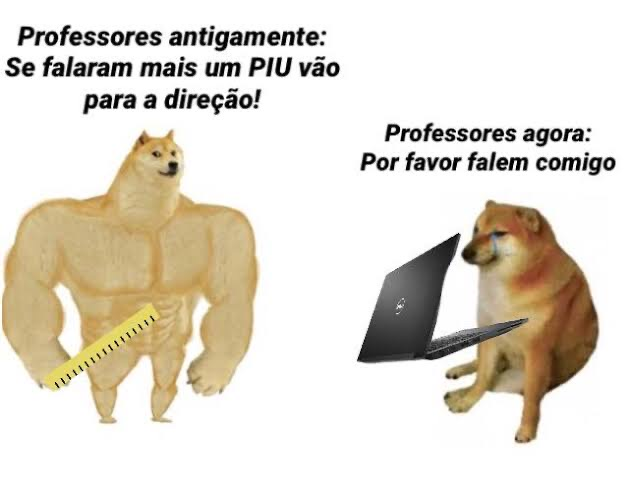
\includegraphics[width=\textwidth]{a46126Texto20do20artigo1489961706781120230920-img002.jpg}
\caption{\textit{Meme} polemizando veladamente com o discurso pedagógico tradicional}
\label{fig:fig2}
\source{Arquivo pessoal.}
\end{minipage}
\end{figure}	
	
O segundo \textit{meme} em análise (\Cref{fig:fig2}) foi produzido, ao que tudo indica, para o público da educação básica, possivelmente alunos e professores dessa etapa de escolarização. As imagens do \textit{meme} são duas e possuem diferentes dimensões. A imagem à esquerda é maior e se destaca no plano imagético em relação a imagem à direita. Acima de cada uma delas estão articulados os elementos verbais do enunciado: a voz de um professor de antigamente, registrada em uma fonte maior, e a voz de um professor de agora, no ensino remoto emergencial, registrada em uma fonte menor. A partir dessa articulação, na qual o visual nasce separado do verbal \cite{lima2022reflexao}, uma vez que as imagens dos animais circulavam na internet antes do ERE, o autor acrescenta não apenas o texto, como discutido no referencial teórico, mas também acrescenta três outras imagens ao enunciado: a régua na mão do cachorro mais forte e o computador e as lágrimas na imagem do cachorro mais fraco. Esses elementos, juntos, serão essenciais para a produção de (novos) efeitos de sentido. Vejamos.
	
A primeira imagem é a de um cão forte, talvez, por isso, uma imagem maior, representando o professor de antigamente, durante o ensino presencial, pondo essa prática, portanto, em destaque. O cão segura uma régua, elemento visual acrescentado pelo autor do \textit{meme}, que pode representar, além de um comum objeto utilizado por professores, uma ação docente ligada ao castigo e à punição, como era o caso do uso da palmatória, que poderia ser substituído por uma régua nas práticas educacionais brasileiras de outrora. A imagem se articula com o dizer “Se falaram [sic] mais um PIU vão para a direção”. Nesse sentido, temos refratada a voz de um professor forte e seguro de sua autoridade, que impede os alunos de falarem durante as suas aulas. Caso os alunos falem pelo menos um “PIU” (note-se o uso da caixa alta que pode representar visualmente um grito do professor) são punidos com a sua retirada da sala de aula e encaminhados à direção. As relações dialógicas entre a imagem do cachorro e a voz do professor nos levam a uma interpretação da presença de um discurso pedagógico tradicional, que pode ser fortemente marcado pela figura de um professor autoritário e ameaçador, assumindo, no plano visual do \textit{meme}, uma posição de destaque. Nesse discurso, o professor geralmente é visto como o centro da aula; os alunos quase nunca são encorajados a participar e a aula pode se dar em forma de monólogo, resultando, como efeito, em um cenário com pouco espaço para a interação e o diálogo.
	
A segunda imagem é a de uma cadela da raça Shiba Inu, que atende pelo nome de Kabosu, conhecida por sua docilidade nas fotos virais que circulam nas redes sociais. Devido ao seu comportamento simpático, o animal acabou compondo os \textit{memes} que comparam dois tipos de comportamento, geralmente um do passado e outro de agora, como acontece no \textit{meme} em análise. A cadela está chorando em frente a um computador, representando o professor de agora, e a imagem se articula com o dizer “Por favor falem comigo”. Nesse caso, a voz é a de um professor frágil e inseguro diante do ERE. Diferentemente da primeira situação, no ERE, o professor quase que implora pela participação dos alunos por meio da expressão “por favor falem comigo”, com destaque para o uso do sintagma “por favor”, imprimindo um tom de desespero no dizer do professor. Diante da realidade do ensino remoto, certas práticas de ensino foram ressignificadas. A falta de participação dos alunos nas aulas \textit{on-line}, devido a problemas técnicos, à ausência de microfone ou, ainda, a dificuldades de conexão com a internet, como verificado em \textcite{bastos2021interacoes}, demandaram dos professores uma nova atitude, qual fosse, o pedido pela participação dos alunos nas aulas, o que polemiza, certamente, com as práticas pedagógicas mais tradicionais, evidenciadas na articulação das duas imagens do \textit{meme}.
	
Ainda é importante pontuar que a reflexão disparada por meio do \textit{meme}, no tocante aos dois tipos de professores, não restringe o debate sobre as práticas educativas tradicionais serem restritas a um professor de antigamente, apenas. Esse modelo, na imagem, tem muito a ver, também, com as posturas docentes em conflito entre \textit{on-line} x \textit{off-line}. A imagem sugere que, apesar de serem antigas, as práticas pedagógicas tradicionais não necessariamente desapareceram das escolas antes da pandemia. O que quero salientar é que mesmo os professores que exerciam um poder disciplinar, por meio do controle e da punição no \textit{off-line}, como destacado pela imagem do \textit{meme}, no ERE, foram confrontados com a necessidade de uma nova forma de interação com os alunos, o que, por sua vez, gerou, como vemos na segunda imagem, um sentimento de fragilidade nas interações \textit{on-line}.
	
No embate entre essas duas vozes refratadas pela inter-relação entre os elementos verbais e visuais, é possível apontar para a possibilidade de o autor estabelecer um efeito de sentido resultante do contraponto dos dois tipos de professores: o professor seguro e autoritário do ensino presencial (o \textit{off-line)} e o professor inseguro e frágil do ensino remoto (o \textit{on-line)}. Tal relação escancara, por meio do humor e da ironia, uma crítica ao comportamento autoritário dos professores no ensino presencial. Esse é o contraponto necessário, em minha interpretação, para estabelecer uma polêmica velada a respeito das práticas tradicionais nas escolas, como a punição aos alunos que questionam, em alguma medida, a autoridade do professor. O discurso do autor do \textit{meme} é, portanto, hostil a um aspecto do discurso pedagógico tradicional, entendido aqui como aquele em que se divulga, dentre outras, a ideia de que o aluno deve ser passivo no processo de aprendizagem, mantendo-se em silêncio. Mesmo sem mencioná-lo diretamente, o autor do \textit{meme} polemiza veladamente com tal discurso, justamente por meio da articulação entre os planos de expressão verbal e visual \cite{brait2013olhar}, como discutido.
 
\begin{figure}[h!]
\centering
\begin{minipage}{.8\textwidth}
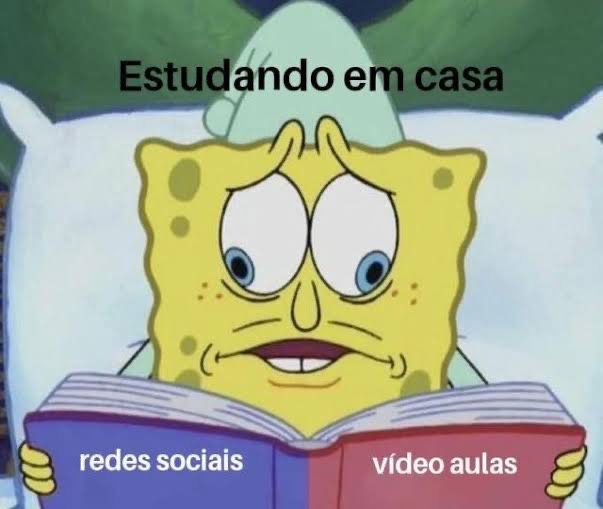
\includegraphics[width=\textwidth]{a46126Texto20do20artigo1489961706781120230920-img003.jpg}
\caption{\textit{Meme} polemizando veladamente com o discurso tecnológico.}
\label{fig:fig3}
\source{Arquivo pessoal}
\end{minipage}
\end{figure}
 
O terceiro e último \textit{meme} (\Cref{fig:fig3}) que trago para a análise é composto por uma imagem, que ocupa o lugar central, e por três elementos verbais. Como nos ensina \textcite{brait2013olhar}, a leitura desse enunciado precisa levar em consideração a articulação desses elementos, uma vez que eles se dão a ler/ver simultaneamente. O enunciado apresenta, como elemento visual, a foto do personagem de desenho animado Bob Esponja. Ele está deitado em uma cama, note-se a presença de um travesseiro atrás de sua cabeça, segurando um livro, olhando, simultaneamente, em direções opostas, para as páginas da direita e da esquerda, o que pode provocar um efeito de sentido de indecisão sobre o que ler primeiro. Na página à direita, encontramos o dizer “redes sociais” e na página à esquerda, o dizer “vídeos aulas”. O livro tem duas cores, azul à direita e vermelho à esquerda.
	
Os dois elementos verbais se articulam, também, a um terceiro que está centralizado acima da imagem “Estudando em casa”. Durante o ERE foi bastante comum, além das aulas síncronas \textit{on-line}, a utilização de vídeoaulas gravadas e disponibilizadas em plataformas digitais aos alunos \cite{bastos2021interacoes}. O \textit{meme} põe em evidência, com isso, que em casa, diante do celular, que ocupa o lugar do livro físico, o aluno pode ter sua atenção facilmente atraída para as redes sociais, mesmo que o ERE demande uma atenção especial às aulas remotas.
	
Se, por um lado, ficar em casa, deitado na cama, como representado na imagem, parece ser mais confortável e, por isso, mais viável para o estudo, por outro lado, as redes sociais disputam lado a lado a atenção dos alunos em relação às videoaulas. Podemos sugerir, então, que a expressão facial um tanto quanto confusa do personagem carrega um tom de preocupação e, certamente, de desconforto com a situação. Essa leitura do \textit{meme} pode nos encaminhar no entendimento de que a voz do autor do enunciado esteja polemizando veladamente com um aspecto do discurso tecnológico, aqui compreendido como aquele que se coloca capaz de melhorar a qualidade do sistema educacional brasileiro sem problematizar, contudo, como as diferentes subjetividades irão reagir ao uso dessas tecnologias, especialmente quando substituem uma prática social como a escola e a sala de aula, como vivenciado no ERE.
	
Cabe salientar que, durante os últimos 20 anos, com o advento da internet 2.0, multiplicaram-se pesquisas acadêmicas insistindo no fato de que o uso das tecnologias digitais da comunicação e da informação, no processo educativo, seriam possibilidades de melhoria do processo educativo (para um estado da arte sobre essas pesquisas ver, por exemplo, \textcite{menezes2019tecnologias}). Contudo, o \textit{meme} parece hostilizar justamente essa ideia divulgada pelo discurso tecnológico, mesmo sem citá-la de maneira direta. O simples fato de o aluno ter um celular e acesso à internet não garante, por meio dos efeitos de sentido produzidos pelo \textit{meme}, que ele conseguirá explorar as potencialidades da tecnologia em favor do seu processo de aprendizagem. Por isso, o \textit{meme} parece manter relação dialógica de concordância com a crítica em torno da falta de formação continuada de professores sobre o uso de tecnologias digitais. Subtende-se, portanto, que faltaram orientações aos alunos sobre a melhor forma de tornar o celular e a internet aliados do processo de ensino-aprendizagem, para que assim, como adiantaram \textcite{paes2020trabalho}, os alunos aprendessem a manusear essas ferramentas para fins educativos.
	
Para finalizar, cabe reafirmar que, pela constituição do discurso \textit{bivocal} do tipo polêmico, exemplificado nos três exemplos de análise acima, o discurso do outro (discurso capitalista, discurso pedagógico tradicional e discurso tecnológico), mesmo sem ser citado no discurso do autor do \textit{meme} de maneira direta, é, de certa forma, atacado e hostilizado. Perceber as sutilezas das relações dialógicas do tipo polêmica velada em discursos do mundo da vida é, por fim, uma das formas de se compreender como as relações dialógicas – relações entre sujeitos via discurso – podem materializar-se em um enunciado (verbo-visual) concreto
	
	
	
\section{Conclusão}\label{sec-conclusão}
	
Como anteriormente anunciado, o objetivo deste artigo foi analisar a polêmica velada veiculada por \textit{memes} a respeito do ensino remoto emergencial, vivenciado durante a pandemia de COVID-19 no Brasil. Verificou-se, em três \textit{memes} analisados, a polêmica velada como maneira de hostilizar, mesmo que de forma subentendida, aspectos dos denominados discursos capitalista, pedagógico tradicional e tecnológico, colocados em relação dialógica com o ERE por meio do projeto de dizer do autor do \textit{meme}.
	
Dessas relações dialógicas, são produzidos sentidos, efeitos de sentidos, que vão em direção a uma crítica social mais ampla, denunciando tanto as fragilidades do ensino remoto emergencial quanto as desigualdades sociais que dificultaram a sua viabilidade. Além disso, a ausência da democratização do acesso à internet e às próprias ferramentas tecnológicas, como o computador, dialoga com as desigualdades estruturais da sociedade brasileira, sustentadas pela força do discurso capitalista, atacado pelo \textit{meme}. Além disso, ao polemizar veladamente com o discurso pedagógico tradicional e com o discurso tecnológico, o autor do \textit{meme} evidencia, por um lado, a insegurança dos professores diante da situação emergencial, e, por outro lado, a dificuldade das ferramentas tecnológicas em afetarem positivamente o processo de ensino-aprendizagem dos alunos. Podemos sugerir, portanto, que os sentidos produzidos pelos \textit{memes} colocam em jogo o (in)sucesso do ERE.
	
Por fim, este estudo, além de registar os sentidos produzidos pelos \textit{memes} analisados a respeito do ERE, coloca-se para a área como mais uma forma de contribuir para sustentar a tese de que a análise da polêmica velada pode ser produtiva no estudo de discursos de diferentes campos da atividade humana, inclusive do campo educacional. Além disso, foi possível indicar como essa categoria pode funcionar em enunciados verbo-visuais a exemplo dos \textit{memes}. Resta saber se seriam os \textit{memes}, por sua peculiaridade de provocar efeitos de humor e ironia, enunciados que sempre polemizam veladamente com outro discurso como parte orgânica de sua arquitetônica. A resposta para essa pergunta, no entanto, escapa dos limites deste artigo.
	
\printbibliography
	
\end{document}

